


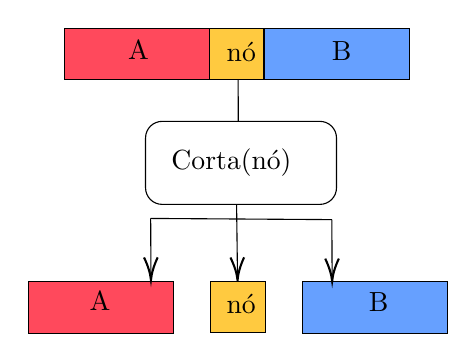
\begin{tikzpicture}[x=0.75pt,y=0.75pt,yscale=-1,xscale=1]
%uncomment if require: \path (0,300); %set diagram left start at 0, and has height of 300

%Rounded Rect [id:dp17006798515443122] 
\draw   (366.1,81.37) .. controls (366.1,76.95) and (369.68,73.37) .. (374.1,73.37) -- (450.1,73.37) .. controls (454.51,73.37) and (458.1,76.95) .. (458.1,81.37) -- (458.1,105.37) .. controls (458.1,109.79) and (454.51,113.37) .. (450.1,113.37) -- (374.1,113.37) .. controls (369.68,113.37) and (366.1,109.79) .. (366.1,105.37) -- cycle ;
%Straight Lines [id:da9040270232690516] 
\draw    (410.71,53.29) -- (410.78,73.17) ;
%Straight Lines [id:da5000031479986659] 
\draw    (409.96,113.35) -- (410.4,147.86) ;
\draw [shift={(410.43,149.86)}, rotate = 269.27] [color={rgb, 255:red, 0; green, 0; blue, 0 }  ][line width=0.75]    (10.93,-3.29) .. controls (6.95,-1.4) and (3.31,-0.3) .. (0,0) .. controls (3.31,0.3) and (6.95,1.4) .. (10.93,3.29)   ;
%Shape: Rectangle [id:dp9336815212866543] 
\draw  [fill={rgb, 255:red, 255; green, 73; blue, 92 }  ,fill opacity=1 ] (327,28.5) -- (397,28.5) -- (397,53.25) -- (327,53.25) -- cycle ;
%Shape: Rectangle [id:dp4996871048748288] 
\draw  [fill={rgb, 255:red, 102; green, 160; blue, 255 }  ,fill opacity=1 ] (423.17,28.5) -- (493.17,28.5) -- (493.17,53.25) -- (423.17,53.25) -- cycle ;
%Shape: Rectangle [id:dp5861288763432269] 
\draw  [fill={rgb, 255:red, 255; green, 73; blue, 92 }  ,fill opacity=1 ] (309.58,150.7) -- (379.58,150.7) -- (379.58,175.45) -- (309.58,175.45) -- cycle ;
%Shape: Rectangle [id:dp3848827559612372] 
\draw  [fill={rgb, 255:red, 102; green, 160; blue, 255 }  ,fill opacity=1 ] (441.58,150.7) -- (511.58,150.7) -- (511.58,175.45) -- (441.58,175.45) -- cycle ;
%Shape: Rectangle [id:dp37173845609371503] 
\draw  [fill={rgb, 255:red, 255; green, 202; blue, 64 }  ,fill opacity=1 ] (397,28.5) -- (423.17,28.5) -- (423.17,53.25) -- (397,53.25) -- cycle ;
%Shape: Rectangle [id:dp5801418703358182] 
\draw  [fill={rgb, 255:red, 255; green, 202; blue, 64 }  ,fill opacity=1 ] (397.57,150.5) -- (423.74,150.5) -- (423.74,175.25) -- (397.57,175.25) -- cycle ;
%Straight Lines [id:da37010559457620107] 
\draw    (368.57,120.14) -- (455.86,120.71) ;
%Straight Lines [id:da7130170295917732] 
\draw    (368.57,120.14) -- (368.7,147.86) ;
\draw [shift={(368.71,149.86)}, rotate = 269.72] [color={rgb, 255:red, 0; green, 0; blue, 0 }  ][line width=0.75]    (10.93,-3.29) .. controls (6.95,-1.4) and (3.31,-0.3) .. (0,0) .. controls (3.31,0.3) and (6.95,1.4) .. (10.93,3.29)   ;
%Straight Lines [id:da8330213784874337] 
\draw    (455.86,120.71) -- (455.99,148.43) ;
\draw [shift={(456,150.43)}, rotate = 269.72] [color={rgb, 255:red, 0; green, 0; blue, 0 }  ][line width=0.75]    (10.93,-3.29) .. controls (6.95,-1.4) and (3.31,-0.3) .. (0,0) .. controls (3.31,0.3) and (6.95,1.4) .. (10.93,3.29)   ;

% Text Node
\draw (356.48,33.19) node [anchor=north west][inner sep=0.75pt]   [align=left] {A};
% Text Node
\draw (454.58,33.45) node [anchor=north west][inner sep=0.75pt]   [align=left] {B};
% Text Node
\draw (377.34,85.32) node [anchor=north west][inner sep=0.75pt]   [align=left] {Corta(nó)};
% Text Node
\draw (337.95,154.17) node [anchor=north west][inner sep=0.75pt]   [align=left] {A};
% Text Node
\draw (472.46,154.71) node [anchor=north west][inner sep=0.75pt]   [align=left] {B};
% Text Node
\draw (403.96,33.85) node [anchor=north west][inner sep=0.75pt]   [align=left] {nó};
% Text Node
\draw (403.87,155.19) node [anchor=north west][inner sep=0.75pt]   [align=left] {nó};


\end{tikzpicture}

